\documentclass[conference]{IEEEtran}
\IEEEoverridecommandlockouts
% The preceding line is only needed to identify funding in the first footnote. If that is unneeded, please comment it out.
\usepackage{cite}
\usepackage{amsmath,amssymb,amsfonts}
\usepackage{algorithmic}
\usepackage{graphicx}
\usepackage{textcomp}
% \usepackage{xcolor}
\bibliographystyle{IEEEtran}
\usepackage[table, dvipsnames]{xcolor}

\begin{document}

\title{Characterization of Patterns in Deep Learning Models using eBPF\\
}

\author{\IEEEauthorblockN{André Lucena Ribas Ferreira}
	\IEEEauthorblockA{
		\textit{University of Minho}\\
		Braga, Portugal \\
		pg52672@uminho.pt}
	\and
	\IEEEauthorblockN{Carlos Eduardo da Silva Machado}
	\IEEEauthorblockA{
		\textit{University of Minho}\\
		Braga, Portugal \\
		pg52675@uminho.pt}
	\and
	\IEEEauthorblockN{Gonçalo Manuel Maia de Sousa}
	\IEEEauthorblockA{
		\textit{University of Minho}\\
		Braga, Portugal \\
		pg52682@uminho.pt}
}

\maketitle

\begin{abstract}
    Deep learning has seen a massive increase in usage in recent years. Often, the bottleneck in these types of workloads is I/O and because of this a large body of work has gone into 
    the characterization of training workflows however these don't get down to the lower levels of the kernel and therefore lack some depth. eBPF have gained popularity for being a way
    of running user space code on the kernel which allows for more in-depth data data gathering. We show that there are novel insights to be gained with the use of these tools.


\end{abstract}

\begin{IEEEkeywords}
     DeepLearning, ResNet50, AlexNet, Pytorch, Characterization, eBPF
\end{IEEEkeywords}

\section{Introduction}
In recent years Machine Learning has seen a massive increase in popularity.
Specifically, Deep Learning (DL) has been used extensively in several modern Computer Science tasks such as image classification
and natural language processing.
Due to these applications' I/O bottlenecks \cite{beegfsDL}, there have been several studies that analyze the I/O patterns of DL Workflows, whose work
has been used to produce useful assumptions about DL I/O patterns. These have been commonly used to
justify various types of optimization explorations (\cite{LMDB, nvme, beegfsDL, bamboo}), and inform
other applications, such as benchmarks specific to DL (\cite{TFbenchmark, OanaDL}).
Application-specific I/O characterization is therefore a requirement for creating
unique and worthwhile solutions to
newer performance problems, as well as, for example, reducing the monetary cost of training an
DL model \cite{bamboo}. However, very few of the existing I/O characterization tools
can get down to the kernel level, instead opting, for example for intercepting system calls using \texttt{LD\_PRELOAD} \cite{HPCIODarshan}. This approach leaves out important information on what is actively occurring at levels closer to the operating system.

There are several ways to interact with the kernel at a low level, such as modifying the kernel source code or using kernel modules. While direct modifications offer efficiency and a high degree of customization, maintaining these changes across different kernel versions and configurations poses significant challenges due to the need for repeated compiling, testing, and adaptation. One technology that has gained significant traction in recent years is the extended Berkeley Packet Filter (eBPF).
eBPF allows for the safe execution of customized kernel code by injecting user-space code into the kernel at runtime.
This eliminates the need for rebooting the system or modifying the kernel source code.
Initially designed for network-related use cases as BPF, eBPF has expanded to support a wide range of applications, including network traffic analysis and filtering, security, tracing, and profiling across various levels of the kernel \cite{eBPFSurvey2}.

Existing tools, such as those developed using bpftrace, a high-level language that abstracts some underlying eBPF logic, can be injected into various parts of the kernel to trace diverse targets,
such as CPU, memory, disk, the virtual file system, and network.
Our goal is to show that eBPF tooling has the possibility to provide an innovative I/O characterization. To that end, we leveraged and modified these tools to collect data at different kernel levels and gather statistics useful for the characterization of DL training workflows.

Besides that, eBPF's also bring some new challenges, so it is crucial to evaluate the overhead and limitations of these tools, to determine which are most suitable for our study and understanding the appropriate layers and points within the kernel where they should be applied.

\textbf{Contributions.} The main contributions of this paper are as follows:
\begin{itemize}
	\item Provide a methodology for characterization of DL, including methods for collecting data using existing and custom tools based on eBPF's, and tools to gather and visualize the collected data.
	\item Provide useful insights about the patterns of certain DL workflows based on an analysis of the collected data, as a Proof of Concept of the variety of insights that may be collected this way.
\end{itemize}

% \begin{itemize}
% 	\item Machine learning has increased in popularity
% 	\item Deep Learning is a subset of Machine Learning
% 	      \begin{itemize}
% 		      \item image classification
% 		      \item natural language processing
% 	      \end{itemize}
% 	\item studies have tried to analyze I/O patterns in DL Workflows (source)
% 	\item \item I/O Characterization has served to produce diverse assumptions about DL I/O behavior, like high overhead for random reads, which are commonly used to justify various types of optimization explorations (\cite{LMDB}, \cite{nvme}, \cite{beegfs}), and inform other applications based on them, like benchmarks specific to DL \cite{TFbenchmark}. Application-specific storage characterization is required to find unique and worthwhile solutions for newer performance problems.
% 	\item very few get down to kernel level
% 	\item eBPF are ...
% 	\item we seek to provide a tool to Characterize DL workloads using eBPF's
% \end{itemize}

\section{Background}

% passing the chosen data as input through the entire network layer by layer, a method called the forward pass. Afterwards, a chosen loss function compares the difference the network's output and the known ground truth, and the gradient of this function is computed in regard to the network's weights. This step is named backpropagation. The gradients are then used to update the weights of all the layers, converging to a minimization of the loss function, through an algorithm called Gradient Descent, that uses the entire dataset as the input. Each pass of the entire dataset is called an epoch, and several are computed in order to converge to the minimum. \cite{gradient} acho que isto está muito grande e fala pouco do I/O

%However, this approach is extremely costly due to the aforementioned dimension of the dataset, so state-of-the-art algorithms use Stochastic Gradient Descent (SGD) instead, an approximation that breaks an epoch into iterations, that go through the only a subset of the dataset, called a \textit{mini-batch}, as input, ensuring that each data sample is iterated through only once \cite{sgd}. Even if the original SGD only fetches a single data sample per iteration, the number of samples has been increasing over the last years, from 32, to 256 and ultimately to the 80.000s, in order to better utilize the increasing computational power afforded by the widespread utilization of GPUs as accelerators, but at an increased I/O load per iteration \cite{nvme}.

In this section, we elaborate on both the Deep Learning algorithms we seek to analyze, with focus on their I/O description, and the eBPF tools we'll use for that end.

\subsection{Deep Learning}

Deep learning (DL) is a subset of machine learning, characterized by its bigger size and heterogeneity of both algorithms and training datasets, needed for accurate predictions \cite{gradient}. State-of-the-art DL utilizes the Stochastic Gradient Descent (SGD) method, which consists in breaking down sequential training epochs in iterations, wherein subsets of the entire dataset, called \textit{mini-batches}, are read, preprocessed in memory and fed to the algorithm. To reduce training time, this computation may be done in accelerators, like GPUs, and may also be overlapped by the parallel I/O of future batches. For maximum accuracy, each data sample is iterated through only once in each epoch and each batch is shuffled, that is, it is composed of random data samples.

To further accelerate the training process, the dataset can be distributed among several workers in Distributed Deep Learning (DDL). When partitioning data, the model parameters are cloned among all the workers, each of them iterates through a subset of the data, and then the gradients are averaged and shared with all the workers. This way, all replicas of the network are updated with the same gradients, ensuring all workers remain consistent with each other.

As models get larger and more nodes are used in training, especially in High Performance Computing (HPC) centers, fault tolerance becomes an important issue. To address it, it is common for the model state to be saved periodically to persistent storage. Normally, this is done at epoch boundaries \cite{checkfreq}, which stalls the algorithm, waiting for I/O. In case of failure, the model state can be loaded from storage and training can be restarted.

Various frameworks exist to facilitate the implementation of DL models, and each one tackles I/O differently. \textit{Pytorch} \cite{pytorch} is an up-and-coming open source AI training library, reportedly becoming commonplace in HPC centers. It provides utilities for operating on tensors with GPU support; various customizable data loading and checkpointing specifications, like parallel data treatment by different workers; a library of ready-to-use DNN models; and support for data parallel training of AI models. Its data structure is analogous to those used in other frameworks, like Tensorflow, and common databases used for DL, like LMDB, as it is based on NumPy, which uses memory mapping for its metadata access \cite{LMDB}.

\subsection{I/O in Deep Learning}

DL's I/O patterns have been attributed as the cause for the increasing storage bottleneck found recently in these applications \cite{beegfs}. On the one hand, the usual dataset's average sample is very small, but also very numerous. For example, 75\% of ImageNet's samples are smaller than 147 KB, while the dataset itself consists of over 14 million images. Allied with the random choosing of samples for batches and the scan nature of each epoch's full dataset traversal, these patterns don't allow for the typical optimizations of traditional storage systems, directed at large and sequential patterns, like prefetching and caching \cite{initial}. On the other hand, the number of samples used for each batch has been increasing over the last years, from 32, to 256 and, in some cases, to the 80.000s, in order to better utilize the higher computational power \cite{nvme}. This comes at an increased I/O load per iteration, while also reducing the overlap between I/O and computation, as GPU utilization tends to scale better than I/O performance when the input sizes are bigger \cite{TFbenchmark}.

Although DL is based primarily upon a read workload, when checkpointing is enabled there are moments of heavy writes. Checkpointing sizes depend on the size of the network, as they can be defined with wholly different numbers of layers and weights, which impacts differently the overall distribution.

\subsection{eBPF}

\textit{Extended Berkeley Packet Filter} (eBPF) is a technology that has attracted massive adoption by both industry and academia, with a wide range of applications such as network, storage, security and sandboxing.
The main advantages are being able to run programs in kernel without modifying the kernel source code nor rebooting the system in order to take effect \cite{eBPFSurvey}.
It is possible to trace different kernel layers while having distinct targets such as CPU, memory, disk and the file system by using different hook points along the Linux Kernel.

Early on, creating and managing eBPF programs would require profound insights into the Linux Kernel and familiarity with low-level programming languages to generate eBPF bytecode,
to facilitate the creation, compilation and execution of eBPF programs, bpftrace \cite{bpftrace}, a high-level tracing language inspired in DTrace and awk allows writing intuitive and efficient eBPF scripts,
reducing the burden of low-level programming and simplifying the act of probing system behavior in a more high-level fashion. \cite{eBPFSurvey2} 

Bpftrace can be used alongside a wide range of tools, many of which are provided by its developers. Additional tools and resources can also be found in \cite{bgreggBook}.

\section{Related work}

% Machine Learning in and out of HPC

HPC centers' wide array of hosted scientific applications has fostered a need for quality and application agnostic I/O pattern identification. Other studies have developed tools for that end, like Darshan \cite{HPCIO24/7}, that seeks to transparently, through \texttt{LD\_PRELOAD}, classify the per-file access statistics of different processes of a given application, while minimally impacting the system it is running on. Various more specialized approaches have built upon Darshan as a base, in order to better depict a distributed environment. These include Wang et al. \cite{zoomin} and their top-down analysis, from system-wide, using HPC's specific monitoring tools Lustre Monitoring Toolkit and Slurm Logs, to single-job, using Darshan, while also introducing two techniques for I/O analysis, a correlation matrix between runs with different parameters and sweep-line based analysis of file access bottlenecks; or Darshan's own HPC focused enhancement \cite{HPCIODarshan}.

However, with DL applications gaining ground in HPC centers, studies have adapted to specific analysis of their I/O traits. Some have kept Darshan as their backbone, either to conduct general DL pattern descriptions, with focus on HPC's response to those workloads (\cite{IOHPCDLBOOK,CharacterizationMLIOLeadHPC, UnderstandingDLIOHPC}), or to develop more advanced tools for that end (\cite{DFTracerAIHPC}). TF-Darshan \cite{tfdarshan} is one of those tools, transparently integrating Darshan with the DL framework Tensorflow's own profiler TensorBoard through runtime linkage, although it doesn't integrate with any other DL frameworks. Others sought to explore the performance bottlenecks around DL's data usage, be it at the database level, for example, LMDBIO \cite{LMDB}, a proposed optimization for LMDB, one of the most used DL databases, and its \texttt{mmap} and randomization related shortcomings, or be it at the file system layer, especially considering parallel systems at HPC centers, proposing alternatives like BeeGFS \cite{beegfs} and ways to leverage it towards DL I/O optimization \cite{beegfsDL}.

Due to DL's overwhelming majority of read operations, the most common examined metrics include the I/O file skew and full read time per process; the read bandwidth for each block size and the number of context switches happening on I/O blocked processes. We've identified some gaps in all analysis overall, like the lack of focus on cache utilization during the epoch dataset scan, lack of network characterization in Distributed Learning communication between workers and, most of all, lack of full I/O stack analysis, considering each step of the training process, over time. Additionally, Darshan itself lacks functionality to adequately track \texttt{mmap} based data manipulation, like \texttt{msync} calls, without additional, intrusive extensions \cite{tfdarshan}, which limits their interaction with DL's most used data representation techniques \cite{LMDB}.

% Observation through eBPFs
In terms of eBPF, there are some tools that are used for system tracing and performance analysis,
such as DIO \cite{DIO} that allow the observation of I/O interactions between the application and in-kernel storage,
\cite{CAT} which is able to correlate the flow of storage and network requests application and \cite{tracee} that provides runtime security and forensics.

% Machine Learning analysis with eBPFs
There are already some studies that use eBPF's capability to provide kernel-level information to understand patterns, such as \cite{eBPFDLNetwork} that
leverages eBPF to monitor DDL training, investigating network bandwidth utilization in DDL, without observing many other metrics about its interaction with the I/O system.
eBPF has also been utilized to characterize machine and deep learning workloads, focusing on storage and I/O efficiency in training,
revealing how storage interactions impact overall performance \cite{OanaDL, OanaML}, which produced general observations for a more precise and accurate benchmark for DL.

Considering all previous work, we believe that there is a lack of descriptions of the full impact in the entire I/O stack of DL as a workload, considering all its possible variations, including different batch sizes and using PyTorch as a framework. Existing DL's I/O characterization focuses on either providing tools for analysis, providing benchmarks mimicking DL patterns or resolving a specific problem due to a previous observation. The work that has produced observations hasn't gone as deep into the kernel stack and inner workings and its particularities as we think is needed to provide full and comprehensive insights.

In that sense, we aim to show the utility and capacity of deeper kernel analysis using eBPFs for innovative insights into DL patterns, both for its I/O patterns and for other related system impact, by analyzing representative DL models tools that monitor and trace multiple different kernel activities.

\section{Design}
The system, also described in Figure \ref{fig:Design}, is composed of three main components:
\begin{itemize}
	\item \textit{Collector}. Allows collecting system information during model training.
	\item \textit{Backend}. Offers a method for storing, searching and analyzing the raw data collected.
	\item \textit{Visualizer}. Provides a way to represent the data collected through different graphical formats in order to facilitate the understanding and analysis of complex logs by transforming them into more intuitive visual representations.
\end{itemize}

\begin{figure}[htbp]
	\centering
	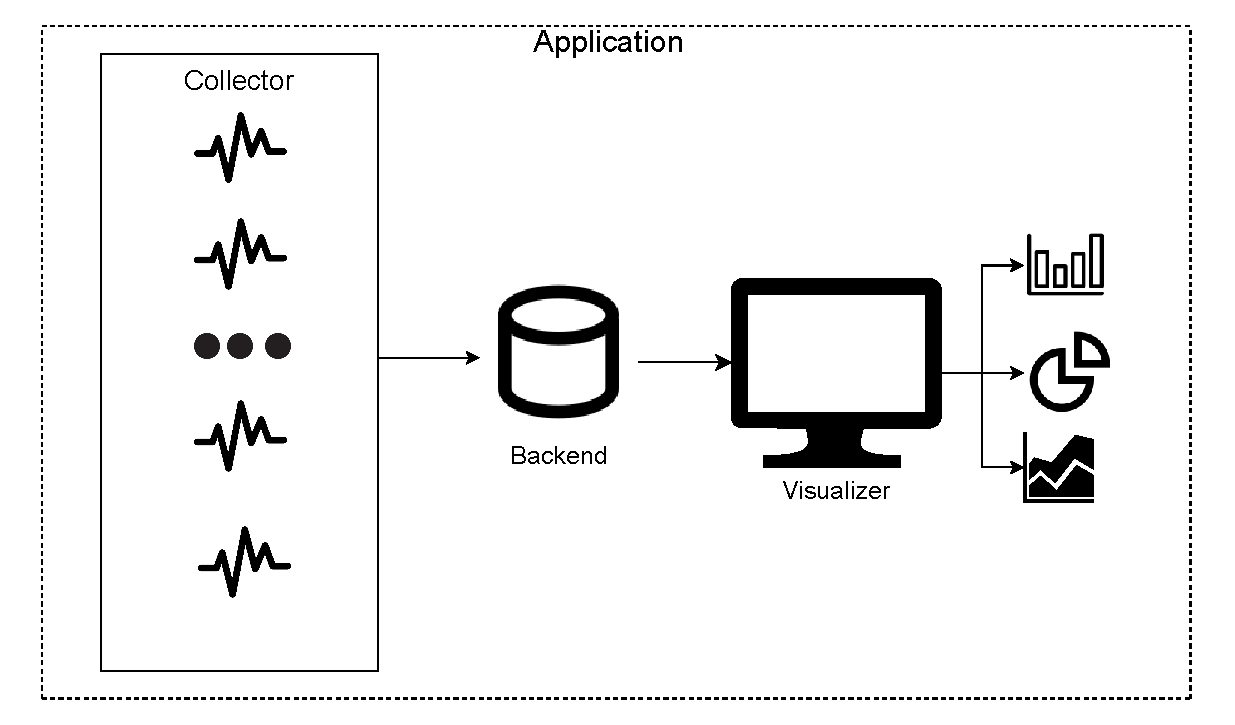
\includegraphics[width=0.45\textwidth]{images/DesignPIV3.pdf}
	\caption{Design}
	\label{fig:Design}
\end{figure}

\section{Implementation}
The implementation of the system is divided into the three main components described in the design section.
There are two versions of the system, each using different approaches for data collection, storing and visualization.

Next we overview a more detailed breakdown of how each component was developed and integrated for both versions.

\subsection{Bpftrace and Python}

\subsubsection{Collector}

For data collection, we used bpftrace\cite{bpftrace} in conjunction with pre-built tools available in the official repository and the following book \cite{bgreggBook}.
However, we modified most of these tools to better suit DL training, as some of them presented all the collected data together, without any time context.
Others were not detailed enough, capturing system-level metrics instead of focusing on the deep learning training process.
Additionally, we created custom eBPF tools to improve data collection and, beyond those, we used the tools \texttt{dstat} and \texttt{nvidia-smi} to, respectively, verify some of our implementations and to monitor GPU utilization, as eBPFs still aren't capable of in-GPU monitoring. We used a GNU Screen \cite{screen} session to allow the scripts to run in the background during long training sessions.

\subsubsection{Backend}

The raw data is stored in the XFS file system, which ensures efficient handling of large datasets, the file system that also hosts our dataset.
We process the stored files by parsing the bpftrace logs, after which the data is aggregated into structured formats for analysis.
Some results are plotted directly for visualization and saved in PDF and HTML formats, while others are stored in pickle format for direct querying or interactive visualizations.

\subsubsection{Visualizer}

For visualizing the data, we use Matplotlib, Seaborn, and Plotly from Python.
Matplotlib and Seaborn are primarily used to generate heatmaps, while Plotly is employed for creating different interactive visualizations.

\subsubsection{Limitations}

Some limitations of this version include the need to build and maintain the entire pipeline using handmade scripts, to connect the different tools and ways of execution.

In addition, if new forms of visualization are required, the parser and visualizer must be adapted to handle different bpftrace log types or generate new types of visualizations.

Other limitations include the scalability of the system, as the dataset size or model complexity increases, the current data collection and processing pipeline may face performance bottlenecks.

Also, the custom modifications made to the bpftrace tools may limit the flexibility of the system, as it could require significant adjustments to apply the pipeline to other models, setups and ML/DL frameworks.

\subsection{Grafana pcp-bpftrace}

\subsubsection{Collector}

The collector is implemented using bpftrace, but the execution of the programs is managed by the pcp-bpftrace extension in Grafana, giving Grafana control over the lifecycle of the programs.

\subsubsection{Backend}

For the backend, we used PCP, which provides a flexible infrastructure for storing, aggregating, and analyzing performance data at scale over time.
It integrates with bpftrace, enabling more granular tracing of specific events via the extension.

\subsubsection{Visualizer}

The visualizer is built on Grafana, which connects to the PCP backend to retrieve performance data and presents it through customizable dashboards.
The use of Grafana allows for real-time, interactive monitoring of system metrics, enabling users to gain insights into the performance of the model training process.

With the pcp-bpftrace extension, it is possible to write bpftrace code directly in Grafana and apply filters and transformations, taking advantage of the wide range of plots that Grafana offers.

Additionally, the extension provides the ability to display flamegraphs, and there is no need to modify the code that collects and presents all the information in one place, since Copilot restarts the bpftrace programs over time.

\subsubsection{Limitations}

We found that this setup does not allow us to collect information and analyze it later, as it is a real-time system.
We would also still need to modify some bpftrace code to make it compatible with the plots in Grafana.

Moreover, we found that the setup difficult due to outdated and incomplete documentation, which created issues with configuration and setup.
It also shares the same limitation as the other version, in that it needs to be adapted for other deep learning frameworks and models.

Finally, some statistics, such as GPU usage, cannot be directly displayed with this extension because they are not gathered with bpftrace. To display these metrics, we would need to use an alternative method in Grafana.

For these reasons, we focus our evaluation on the first implementation we presented.

\section{Evaluation}

\subsection{Experimental Setup}

We analyzed the training of the large network ResNet50 \cite{resnet50} and the smaller AlexNet \cite{alexnet}. Those models were
provided by the \textit{PyTorch} framework, where they're defined with 50 and 13 layers, respectively. Our testing machine is equipped with an Intel® Core™ i9-9900K CPU @ 3.60GHz with
8 physical cores, 16 virtual cores, 16GiB of total RAM and an NVIDIA Corporation TU104 [GeForce RTX 2070 SUPER]. The OS runs Rocky Linux 9.4 (Blue Onyx) with kernel Linux 5.14.0-427.37.1.el9\_4.x86\_64. The dataset we used is the ImageNet \cite{imagenet} dataset, an assemblage of labeled images for the training of image classification models, which is originally comprised of 1.2 million sample images, with an average size of 192KiB and a total size of 240GiB. Due to storage technical limitations, we scaled the dataset down to 45GiB total size (of which 36GiB were used for training) by randomly selecting images. This was done for coherence between this evaluation and a limited Distributed Learning analysis that wasn't concluded by the end of the writing of this paper.

\subsection{Methodology}

We ran a series of experiments with different parameters, in particular these combinations are:
\begin{itemize}
	\item ResNet50 or AlexNet models.
	\item One or two training epochs.
	\item With or without checkpointing.
	\item With or without code generated training logs (marking different training steps).
	\item With 32 and 64 samples of batch size.
\end{itemize}
In order to not have interference between different runs, the operating system's cache was dropped after each run.

A full execution was run for every combination of parameters, which was followed by the processing and analysis of the visualization techniques.
After some analyses of the data further, smaller experiments were conducted, in particular:
\begin{itemize}
	\item Varying the \texttt{num\_workers} parameter of the PyTorch DataLoader, with 0, 1 and 4 workers, testing both models during two epochs, a batch size of 64, no logging, and with a checkpoint at each epoch boundaries.
	\item Dropping the system cache at epoch boundaries.
	\item Changing some eBPF tools, like \texttt{biolatency}, by altering hook points.
\end{itemize}

\subsection{Results}

\begin{table}
    \caption{System calls}\label{tab:syscalls}
    \begin{center}
        \begin{tabular}[c]{|l|l|l|}
            \hline
            \rowcolor{gray}
            Syscall & ResNet50 & AlexNet\\
            \hline
            \rowcolor{lightgray}
            \#1 & sched\_yield & read\\
            \hline
            \#2 & read & lseek\\
            \hline
            \rowcolor{lightgray}
            \#3 & lseek & close\\
            \hline
            \#4 & close & newfstat\\
            \hline
            \rowcolor{lightgray}
            \#5 & newfstat & ioctl\\
            \hline
            \#6 & ioctl & openat\\
            \hline
            \rowcolor{lightgray}
            \#7 & openat & futex\\
            \hline
            \#8 & futex & write\\
            \hline
        \end{tabular}
    \end{center}
\end{table}

\begin{table*}
    \caption{Perf}\label{tab:perf}
    \begin{center}
        \begin{tabular}[c]{|l|l|l|l|l|l|l|}
            \hline
            \rowcolor{gray}
            Model & Epoch & Batch Size & Ckeckpoint & Logging & Time w/ eBPF & Time w/o eBPF \\
            \hline
            AlexNet & 2 & 32 & 1/epoch & false &    33m47.868s & 33m10.190s \\
            \hline
            AlexNet & 2 & 32 & none & true &    34m21.545s & 33m27.275s \\
            \hline
            AlexNet & 2 & 32 & 1/epoch & false &    33m53.268s & 33m10.023s \\
            \hline
            AlexNet & 2 & 32 & 1/epoch & true &    34m55.783s & 33m24.529s \\
            \hline
            AlexNet & 2 & 64 & none & false &    33m43.084s & 33m3.322s \\
            \hline
            AlexNet & 2 & 64 & none & true &    34m13.559s & 33m20.241s \\
            \hline
            AlexNet & 2 & 64 & 1/epoch & false &    33m53.426s & 33m5.216s \\
            \hline
            AlexNet & 2 & 64 & 1/epoch & true &    34m17.983s & 32m58.640s \\
            \hline
            ResNet50 & 2 & 32 & none & false &    57m46.997s & 57m46.194s \\
            \hline
            ResNet50 & 2 & 32 & none & true &     57m46.116s & 57m45.615s \\
            \hline
            ResNet50 & 2 & 32 & 1/epoch & false &    57m43.254s & 57m44.610s \\
            \hline
            ResNet50 & 2 & 32 & 1/epoch & true &     57m46.191s & 57m46.028s \\
            \hline
            ResNet50 & 2 & 64 & none & false &    55m53.568s & 55m49.152s \\
            \hline
            ResNet50 & 2 & 64 & none & true &     55m57.438s & 55m48.515s \\
            \hline
            ResNet50 & 2 & 64 & 1/epoch & false &    55m53.242s & 55m52.361s \\
            \hline
            ResNet50 & 2 & 64 & 1/epoch & true &     55m52.560s & 55m48.773s \\
            \hline
        \end{tabular}
    \end{center}
\end{table*}


\hspace{-0.55cm} \textbf{Observation 1.} Training images are read concurrently by multiple processes on training with several workers.
\\
\textbf{Observation 2.} \texttt{fsync()} is not called by any of the processes created by PyTorch, this means that \texttt{torch.save()} does not call \texttt{fsync()}, confirming the assertion made in \cite{checkfreq}.
\\
\textbf{Observation 3.} The vast majority of system calls performed by ResNet50 (3.7 Billion with 2 epochs and batch size 64) are \texttt{sched\_yield()}. These calls are all made by two threads created by the master process, which runs the main function and schedules the model's training.
\\
\textbf{Observation 4.} Checkpoint data was always written to persistent storage when \texttt{torch.save()} was called, confirmed by checking the block I/O write size.
\\
\textbf{Observation 5.} When reading from a pipe, processes will read in two moments, reading the first byte and then a larger chunk of data. This results in there being approximately twice as many reads as there are writes to pipes, this pattern is persistent even through changes to the \texttt{num\_workers} parameter in the DataLoader class.
\\
\textbf{Observation 6.} The amount of reads and writes to pipes is proportional to the amount of workers allocated in the DataLoader PyTorch class. When no workers are allocated, no reads or writes to pipes are performed.
\\
\textbf{Observation 7.} The pattern of block read operation completions is as follows: a large number of initial operations followed by a gap, i.e., a practically complete drop to near 0 reads, until the end of the first epoch. During the remaining epochs, even to 3 epochs, the accesses are done uniformly.
\\
\textbf{Observation 8.} Before the read gap begins, there is a stabilization of the system memory used as cache, at around 12GiB of usage.
\\
\textbf{Observation 9.} The size of the gap is proportional to the number of worker processes used to read from disk, and so the gap is smaller the fewer workers used. With zero workers, the gap does not exist.
\\
\textbf{Observation 10.} This pattern maintained even when the operating system's cache was dropped between epochs.
\\
\textbf{Observation 11.} Regarding the two hook points used for capturing the block read operation completion, that we assumed were exclusive of each other, when tracing with either one active, the union of the results did not equal the results of having both hook points active by an order of magnitude (10.000s against 1.000s for each one).
\\
\textbf{Observation 12.} The amount and size of block read operations issued to the disk is constant throughout the whole training, even inside the timeframe of the gap, that indicates that no block read operation is completed during that time.
\\
\textbf{Observation 13.} When writing the checkpoint, the process writes using \texttt{writev} system calls, with the final chunk of data written using a \texttt{write} system call.
\\
\textbf{Observation 14.} We found the following system calls correlate to the checkpoint when model training with both models: \texttt{rt\_sigprocmask}, \texttt{mprotect}, \texttt{rmdir}, \texttt{exit\_group}, \texttt{rt\_sigreturn}, \texttt{getdents64}, \texttt{madvise}, \texttt{wait4}, \texttt{exit}, \texttt{clone3}, \texttt{rseq}, \texttt{rt\_sigaction}, \texttt{writev}, \texttt{waitid}, \texttt{gettid} and \texttt{set\_robust\_list}.
\\
\textbf{Observation 15.} We found the following vfs functions calls correlate to the checkpoint when model training with both models: \texttt{writev} and \texttt{rmdir}.
\\
\textbf{Observation 16.} Both AlexNet and ResNet50 exhibit a similar hierarchy of system calls, with the notable exception of ResNet50's inclusion of \texttt{sched\_yield} as the first call. The system calls are as follows: \texttt{read}, \texttt{lseek}, \texttt{close}, \texttt{newfstat}, \texttt{ioctl}, \texttt{openat}, \texttt{futex} and \texttt{write}, also see in Table \ref{tab:syscalls}.
\\
\textbf{Observation 17.} Although ResNet50 has a smaller checkpoint size, it performs 209 \texttt{writev} syscalls compared to just 16 by AlexNet.
\\
\textbf{Observation 18.} Both models have CPU run queue empty during the entire duration of model training, which shows no contention between processes.
\\
\textbf{Observation 19.} The run queue latency is similar in both cases, with the interval \([2, 4[\) microseconds being the most dominant, followed by \([1]\), and then \([4, 8[\).
\\
\textbf{Observation 20.} As shown in Table \ref{tab:perf}, the eBPF overhead is comparable to runs without tracing tools during model training with ResNet50. However, for AlexNet, the overhead can result in a difference of slightly more than a minute.
% \subsubsection{Checkpoint data persistence}
% We observed that no calls to fsync() were performed by the python processes, furthermore, the calls that were performed happened either some time before or some time after the checkpoint was performed, confirming the observation made in \cite{checkfreq} that the torch.save() does not guaranty data persistence.
% We observed however that in all tests performed that the checkpoint data was in fact being persisted to disk.

% \subsubsection{System call usage comparison between models}
% We found that the overwhelming majority(3.7B on tests with 2 epochs and batch size of 64) of system calls performed by the python processes during training of the ResNet50 model were sched\_yield(), when looking at the results segregated by thread we found that ... this is not the case for training AlexNet in the same conditions

% \subsubsection{Read and Write patterns on pipes}
% We analyzed the write and read patterns to pipes of the AlexNet model, we found approximately twice as many reads from pipes as there were writes, upon looking into the pattern we noticed that
% each time a pipe was read from, there was an initial read of 4 bytes followed by a subsequent read of more bytes.
% This pattern remained with variations of the num\_workers parameter for the PyTorch DataLoader class, although the number of operations on pipes reduced in proportion to the number of workers. Conclusively, when this parameter was set to zero workers, there were no reads or writes to pipes.

% \subsubsection{Pattern of block I/O access}
% During the first epoch we found numerous initial reads followed by drop up until the moment the second epoch begins, after which there is a uniform pattern of read's.
% This pattern was consistent with changes to the number of epochs, but the length of the initial burst of read's increased as the number of data loading workers decreased (no workers??).
% This pattern also maintained when the operating systems caches were dropped in between epochs

\subsubsection{Summary}

Overall, the analysis shows novel DL characterizations that wouldn't be possible without deep and precise kernel instrumentation. In particular, the issue of the checkpoint as block I/O write size to the disk shows the checkpoint is persisted to disk (Observation 4), but without deeper analysis it isn't conclusive how their persistence is guaranteed by the PyTorch framework (Observation 2), if at all. The block read operation completions gap (Observation 7) is another observation that needs a more comprehensive understanding of kernel functionality, especially the completion of block requests, to pinpoint the functionality at display. We tried to understand it through Observations 8-11, but the inconsistency with Observation 12 is still unexplained.

\section{Conclusion and Future Work}

With this paper we present a bottom-half analysis of the kernel interactions involved into serving a DL application, with focus on their I/O patterns. We collected multiple different statistics, using eBPF-based tools, transparently and with low overhead on the entire application. We presented those collections and analyzed them, where we found unique patterns we tried to explain through deeper dives into kernel functionality. With them, we concluded that this kind of low level observation is required to completely understand the interaction complex algorithms like DL models have with in-place systems like the I/O stack.

Future work will involve scaling up the tests done, not only in terms of dataset and model size, which would require more computational power, but also investing into Distributed Learning, both for Data and Model distribution. eBPF tools permit the tracking of network calls and data transfers, so they aren't limited to tracking only typical disk I/O.

With DL analysis fully complete, there is the need to keep up with DL's latest trends. Large Language Models (LLMs) have taken the world by storm, with the public availability of applications like ChatGPT \cite{chatgpt}, and so the training of these models is looking to become the norm on HPC centers. Their smaller datasets and larger models, as well as their different data consumption patterns, compared to those of traditional DL models, possibly bring different patterns into consideration when such examinations are conducted.

\bibliography{IEEEabrv, refs}

\end{document}
